\chapter{Problem analysis}
\chlab{analysis}

In this chapter, the problems that this thesis project aims to solve are discussed. First, a brief explanation of the chemical concepts used in the project is provided (\secref{chemical}), followed by the interaction design challenges in \secref{id_challenges}.

\section{Chemical concepts}
\seclab{chemical}
As far as this project is concerned, the most important chemistry knowledge that needs to be present is the fact that every material is built up out of molecules, consisting of a set of atoms. Each of these atoms has a certain type, such as hydrogen~($H$) or carbon~($C$). The atoms of a molecule are connected in a specific way, where the connections are called bonds. There can be multiple bonds between the same atoms, creating double or triple bonds. Every molecule has a total charge, which is the sum of the charges of the individual atoms in that molecule.

\begin{wrapfigure}{r}{.4\textwidth}
\vspace{-2em}
\begin{center}
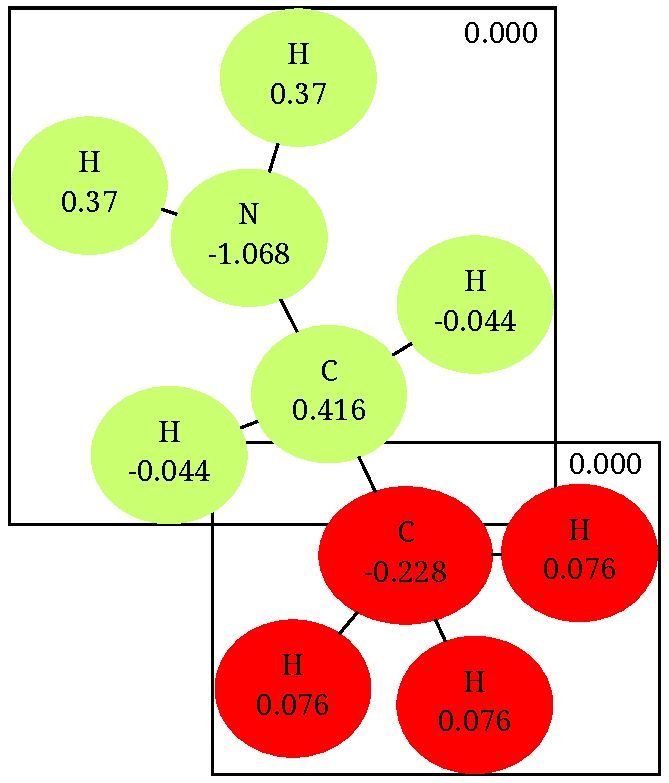
\includegraphics[width=.38\textwidth]{img/ethanamine.pdf}
\caption{Schematic view of ethanamine ($C_{2}H_{7}N$)~\cite{atb2014ethanamine}, including topology data on atom types, atomic charges and charge groups.}
\figlab{partial_charges}
\end{center}
\vspace{-2em}
\end{wrapfigure}

As discussed in the introduction (\chref{introduction}), biomolecular simulations are becoming increasingly important, especially in the field of drug development. For these simulations, force field models are required to describe the interatomic relations of the drug molecules. In order to run a simulation, these force fields require the molecule's topology, which consists of the molecule's atom types, bonds, bond angles, atomic charges and charge groups.

\Figref{partial_charges} shows the schematic view of an ethanamine molecule. Here, every oval symbolises an atom. The atom type is the letter on the top rule of the oval, i.e. $H$ is the atom type of the sphere $H7 (6)$. The first number indicates the index in the list of atoms of that type ($7$ in the example), the second the overall atom index in the molecule ($6$ in the example). The bonds between atoms are shown as lines between the ovals and the atomic charges are given by the number at the bottom row of the oval ($0.37$ for $H7 (6)$). Finally, the colouring of the atoms and the boxes around them denote a charge group. This is a group of connected atoms, for which the total charge is ideally equal to that of the whole molecule ($0.0$ in this example).

In a recent study, El-Kebir, Klau et al. have developed an algorithm that allows for fast and reliable assignment of charge groups~\cite{canzar2012charge}. As this is now optimised, they currently focus on a different step in the parameterisation: that of calculating the atomic partial charges. Currently, these charges are retrieved using complex quantum-mechanical calculations. However, when run on larger molecules, these calculations can take hours or even days to complete. As it is not believed that the algorithms used in these calculations can be improved much further, a different approach is needed for finding atom charges.

As discussed before, a possible approach is to exploit the similarity of molecules and retrieve the partial charges of an unparameterised molecule from similar fragments in other molecules for which the charges \emph{are} known. In \figref{matching}, the basics of fragment matching are shown. In this case, we are looking for a $C$ atom, with three connected $H$ atoms (see \figref{match_1}). \Figref{match_2} shows a matching fragment from a different molecule, that, indeed, consists of a $C$ with three connected $H$s. The fragment shown in \figref{match_3} obviously does not match with the fragment that is being looked for. It does contain two $H$ atoms, but they are connected to an $N$ atom, rather than a $C$. More detailed information on fragment matching can be found in \secref{impl_omfraf}.

\begin{figure}[h!]
\centering
\begin{subfigure}[t]{0.29\textwidth}
\centering
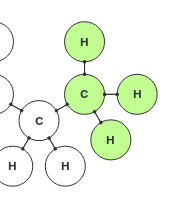
\includegraphics[width=\textwidth]{img/match_1.png}
\caption{Molecule fragment, highlighted in green.}
\figlab{match_1}
\end{subfigure}%
\qquad
\begin{subfigure}[t]{0.29\textwidth}
\centering
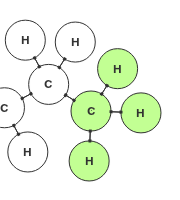
\includegraphics[width=\textwidth]{img/match_2.png}
\caption{Matching fragment, highlighted in green.}
\figlab{match_2}
\end{subfigure}%
\qquad
\begin{subfigure}[t]{0.29\textwidth}
\centering
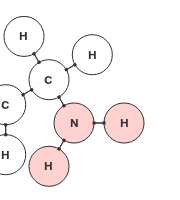
\includegraphics[width=\textwidth]{img/match_3.png}
\caption{Non-matching fragment, highlighted in red / pink.}
\figlab{match_3}
\end{subfigure}
\caption{Basic fragment matching.}
\figlab{matching}
\end{figure}

For an atom, or a set of atoms, usually many matching fragments will be found. Which of those fragments is the best match depends on many factors, including the fragment size and type of molecule they originate from. Due to this, it is currently not possible to fully automate fragment-based parameterisation. Instead, it needs to be done by experienced chemists who have the knowledge about which fragments match well, and which do not. A system is needed that assists them in this process, and allows them to easily compare fragments and molecules.


\section{Interaction Design challenges}
\seclab{id_challenges}
A system for fragment-based molecule parameterisation is not readily available. Therefore, a new system needs to be designed from the ground up. This allows for really creating something new, but also creates the challenge of doing it right without having any clear starting point. Therefore, two different versions of the system will be implemented, in order to find the best way of interacting with such system.

Both implementations need to meet the same set of requirements. First of all, the system needs to provide its users with a view of the unparameterised atom, and help them to find the best matching fragments. As the selected fragments may not always be perfect, it should also be possible for the user to manually adjust the charges for each atom, if he feels that this is needed.

In order to find the best available matching fragment, the user should be able to easily compare the found matching fragments, both with each other and with the unparameterised molecule. He should be encouraged to compare as many fragments as possible, such that he does not miss the best one. When many fragments are found, the best matches should be easily recognisable. Otherwise, fully parameterising the molecule may take up too much time, or that fragment may not be found at all. This requires the found fragments to be presented to the user in a clear and intuitive way.

Another important requirement for the system is that is should support parameterisation of both small molecules, consisting of just a few atoms, and large molecules, being over a hundred atoms in size. This means that visualisation of the molecules should be given some thought, in order to make sure both large and small atoms are displayed correctly. It is particularly challenging to find a way to properly visualise large molecules on a screen with a limited size, so an approach should be developed that allows for this.

Overall, the most important requirement for the system is to make it work intuitively and to implement it such that it makes chemists' work easier. Parameterising a large molecule should therefore not take hours to complete. If it would, chemists would probably still prefer using the conventional quantum mechanical calculations, since one can at least do other things while waiting for those results. When one has to manually parameterise a molecule, this is not possible.
